\chapter{Particle models and simulation of amorphous solids \label{ch:ParticleModels}}

One way to understand macroscopic systems is to trace back their behavior to the particles that constitute them.
Here we describe in detail the features of the Lennard-Jones model, which is the main workhorse used in this thesis to get insights about the mechanical behavior of glassy systems under oscillatory shear. The numerical techniques employed to study it are also presented, with an emphasis on those that aim at describing the behavior of systems under deformation. The most important concept explored in this chapter is the evolution of energy landscapes and inherent structures as strain is changed. This will be the key tool to interpret the results of simulations of LJ systems in \autoref{ch:ParticleModelsResults} and to develop new models in \autoref{ch:ToyModels}.

\section{Lennard-Jones model for glassy systems \label{sec:LennardJonesModel}}

In this thesis, we model glassy systems using an isotropic and pairwise additive potential, as in \cite{utz2000atomistic, lacks2004energy}. More precisely, in what follows we will employ binary mixtures of classical particles interacting via a Lennard-Jones pair potential of the form 
\begin{equation}
	\phi_{\alpha \beta}(r) = 4\epsilon_{\alpha \beta} \left[ \left( \frac{\sigma_{\alpha \beta}}{r} \right)^{12} - \left( \frac{\sigma_{\alpha \beta}}{r} \right)^{6} \right]
	\label{eq:BinaryLennardJonesPotential}
\end{equation}
which has been extensively used in numerical and simulation work to probe and reproduce the behavior of glassy systems.
While a model of this kind cannot reproduce quantitatively the properties of real amorphous materials, it still aims at capturing their behavior at a qualitative level. 

By changing the parameters in \autoref{eq:BinaryLennardJonesPotential}, one can embody in the model two out of the three features listed in \autoref{sec:UndeformedGlasses} that characterize a good metallic glass former. In fact, by varying the value of the matrix $\sigma_{\alpha \beta}$, one varies the range of the repulsive cores of the Lennard-Jones particles, thus changing their effective sizes. By varying the value of $\epsilon_{\alpha \beta}$, instead, one can tune the energy gain obtained when particles of different species are close together. Such value is related to the enthalpy of mixing, which is another key factor that influences glass forming behavior.
Indeed, it has been shown that a careful choice of $\sigma_{\alpha \beta}$ and $\epsilon_{\alpha \beta}$ allows binary Lennard-Jones systems at low temperature to avoid crystallization \cite{toxvaerd2009stability} for a sufficiently long time and exhibit behavior typical of glasses such as a dramatic slowdown of particle diffusion and the breakdown of the Stokes-Einstein relation between viscosity and diffusion in \autoref{eq:StokesEinstein} \cite{bordat2003breakdown}.

\section{Computer simulation of particle systems}

\subsection{Molecular dynamics at constant $E$ or $T$ \label{sec:MolecularDynamics}}

A system of $N$ particles interacting via a pairwise additive potential like that in \autoref{eq:BinaryLennardJonesPotential} has a total potential energy
\begin{equation}
	U(\mathbf{r_{1}, \ldots, r_{N}}) = \sum_{i=1}^{N} \sum_{j<i} \phi(|\mathbf{r_{i} - r_{j}}|)
	\label{eq:TotalPairwiseAdditivePotentialEnergy}
\end{equation}

This value of $U$ can be changed by some amount $\Delta U$ in the presence of an external field (see \autoref{fig:ParticlesInFields}). Moreover, if such a field depends on the position of the particles, then the perturbation can be written as $\Delta U(\mathbf{r_{1}, \ldots, r_{N}})$. 

\begin{figure}[!h]
	\centering
	\begin{subfigure}[b]{0.45\textwidth}
			\centering
			\includegraphics[scale = 0.8]{ParticlesInFields_1.pdf}
			\caption{\label{fig:OpenSystem}}
	\end{subfigure} 
		\begin{subfigure}[b]{0.45\textwidth}
			\centering
			\includegraphics[scale = 0.8]{ParticlesInFields_2.pdf}
			\caption{\label{fig:OpenSystemField}}
	\end{subfigure} \\
		\begin{subfigure}[b]{0.45\textwidth}
			\centering
			\includegraphics[scale = 0.6]{ParticlesInFields_3.pdf}
			\caption{\label{fig:PeriodicBoundaries}}
	\end{subfigure} 
		\begin{subfigure}[b]{0.45\textwidth}
			\centering
			\includegraphics[scale = 0.6]{ParticlesInFields_4.pdf}
			\caption{\label{fig:LeesEdwardsBoundaries}}
	\end{subfigure} \\
\caption{Schematic representation of systems of particles in different environments: 
(\subref{fig:OpenSystem}) interacting particles with open boundary conditions; 
(\subref{fig:OpenSystemField}) interacting particles with open boundary boundary conditions and immersed in a field;
(\subref{fig:PeriodicBoundaries}) interacting particles with periodic boundary conditions. This is a special case of (\subref{fig:OpenSystemField}), but with the field generated by the particles \emph{themselves};
(\subref{fig:LeesEdwardsBoundaries}) interacting particles with Lees-Edwards boundary conditions. This is another special case of (\subref{fig:OpenSystemField}), but with the field generated by the particles. Clearly, in this case the energy of the configuration will depend on the offset in the position of the simulation boxes.
\label{fig:ParticlesInFields}}
\end{figure}

The forces acting on each $i$-th particle are known once that a configuration is specified:
\begin{equation}
	\mathbf{f_i} = - \nabla_{\mathbf{r_i}} U(\mathbf{r_{1}, \ldots, r_{N}})
	\label{eq:Force}
\end{equation}
where differentiation is performed with respect to the coordinates of the $i$-th particle that compose the vector $\mathbf{r_i}$.
If the positions $\{\mathbf{r_i}\}$ and velocities $\{\mathbf{\dot{r_i}}\}$ are specified at a given moment in time $t_0$, the evolution of the system can be determined by integration of the Newton law:
\begin{equation}
	\mathbf{f_i} = m_i \mathbf{\ddot{r_i}} 
	\label{eq:NewtonsLaw}
\end{equation}
In practice, the integration of \autoref{eq:Force} and \autoref{eq:NewtonsLaw} (also called the \emph{$n$-body problem} of classical mechanics) is too hard to be performed analytically even for the simplest interaction potentials if the number of particles is large.  
Fortunately, numerical techniques exist that are able to give approximate solutions of it (these are generally referred to as \emph{molecular dynamics} (MD) methods \cite{allen1989computer, frenkel2001understanding}). The idea behind these methods is to compute the trajectories of the particles by updating their coordinates according to their velocities as time is increased in small discrete intervals of duration $dt$ (timesteps).
One of the simplest and most effective integration schemes is the \emph{velocity-Verlet} scheme \cite{frenkel2001understanding}, which has the desirable property of being time reversible (so that trajectories are retraced if the velocities are reversed at a given moment in time) and of preserving volumes in phase space during the evolution, as required by \autoref{eq:Force} and \autoref{eq:NewtonsLaw} \cite{frenkel2001understanding}.
Such integration algorithms can be implemented using a programming language of choice, so that one is able to simulate the behavior of a system of interacting particles using a computer (or a group of computers).
Nowadays several computer codes that perform the computation above are readily available. In order to do so efficiently, several ``tricks'' can be employed. 
First of all the real systems of interest are usually macroscopic in size, and are thus constituted by a very large number of particles $> 10^{20}$. Dealing explicitly with such a huge number of particles is not possible, as the sheer amount of memory needed to store the positions of such a large set of particles surpasses by far the capacity of ordinary computer systems. 
Luckily, there are ways to partially overcome this. A macroscopic system can be divided in parts (in three dimensions, each of these can be thought as the part of the system contained in a small cubic box, called \emph{simulation box}). To simulate what happens in one of these boxes, one replaces the rest of the system that surrounds it with \emph{identical copies} of it (as displayed schematically in \autoref{fig:PeriodicBoundaries} and \autoref{fig:LeesEdwardsBoundaries}), called ``images''. 
In this way particles at the boundaries of the box ``feel'' an environment that is similar to that that they would experience in the bulk. This is accomplished at a very small cost, that is by computing the additional interactions between particles separated by the boundaries of the box, and applying the so called ``minimum image convention'' \cite{frenkel2001understanding}. This approach is not without drawbacks, as it tends to introduce spurious correlations. However, it can be used to obtain meaningful results by studying a relatively small number of particles (typically, in the range between $10^{2}$ to $10^{6}$).
Note also that the periodic replicas of the particles can be viewed as sources of an external field acting on the particles contained in the simulation box. It's then evident that the boundary conditions do contribute in shaping the features of the potential energy landscape of the system (this is clearly evident in \autoref{fig:LeesEdwardsBoundaries}, where the \emph{exact} same configuration will have a different energy as the offset in the position of the boxes is varied). \\
Another source of problems comes from the fact that the calculation of the forces from \autoref{eq:Force} for a pairwise additive potential like that in \autoref{eq:BinaryLennardJonesPotential} would in principle require the computation of $N(N-1)/2 \approx N^{2}$ forces. The computational complexity of the problem is thus polynomial in $N$, but one would like to have an exponent lower than 2. This is doable by neglecting the interactions between particles separated by a distance which exceeds some cut-off, and thus computing the force acting on a given particle as if it was generated only by the particles closest to it. If a list of neighboring particles can be generated, the complexity is reduced to that of the computation of just $d N$ interactions, where $d$ is the average number of neighbors surrounding each particle. The construction/rebuilding of the lists (cell lists or Verlet lists) \cite{frenkel2001understanding} of neighboring particles often requires less than $N^{2}$ operations or doesn't need to be performed frequently, and thus the overall cost of the computation can be greatly reduced in the case of large systems \cite{frenkel2001understanding}.  

In \autoref{eq:Force}, one assumes that the forces that act on the system are internal, so that it is isolated and its total energy $E = K + U$ (where $K$ is the kinetic energy) is conserved. However, experimental systems are very rarely isolated from their environment. In real experiments what is kept constant is usually the temperature $T$ and the volume $V$ or the pressure $p$ via a contact with an external reservoir and it is crucial to be able to construct simulations capable to match experiments. The naive approach of simulating both the system of interest and a reservoir is too demanding in terms of computational resources to be feasible. For this reason, to deal with systems where the variables $N, V, T$ or $N, p, T$ are kept constant (and sample the canonical and isobaric ensembles respectively), other numerical schemes have been devised, respectively named thermostats and barostats \cite{frenkel2001understanding}. Two popular choices of thermostats for simulations at constant $N, V, T$ are represented by
\begin{itemize}
	\item The Berendsen thermostat
	\item The Nos\'e-Hoover thermostat 
\end{itemize}
Both thermostats are described in \cite{hunenberger2005thermostat}, and aim at making the trajectory of the system visit configuration with a probability compatible with the canonical ensemble \cite{frenkel2001understanding}. In this work the Nos\'e-Hoover thermostat is employed to study systems at a specified temperature $T$.	

\subsection{Simulation of deformation}
Another way (rather than imposing some temperature $T$) to alter experimentally a sample is imposing a deformation on it. An example is a simple shear deformation of the kind described in \autoref{eq:ShearDeformationMatrix}.
Geometrically, such transformation maps a cube with edges parallel to the $x, y, z$ axes onto a rectangular prism whose faces parallel to the $xy$ plane are parallelograms, as depicted in \autoref{fig:SimpleShear}. 

\begin{figure}[!h] 
\centering 
\includegraphics[width=0.8\textwidth]{Shear.pdf} 
\caption{Shear deformation of a rectangular box under the effect of a shear deformation of the kind described in \autoref{eq:ShearDeformationMatrix}, and disregarding the effect on the $z$ direction. The effect of the shear is tilting the box by an angle $\theta$ such that $\tan \theta = \gamma$, and the transformation conserves the volume. \label{fig:SimpleShear}}
\end{figure}

As the determinant of the matrix in \autoref{eq:ShearDeformationMatrix} is equal to 1, the transformation is volume-conserving. 
A macroscopic deformation of this kind can be implemented in a computer simulation by applying the transformation in \autoref{eq:ShearDeformationMatrix} to the simulation box and its images, by means of the so-called Lees-Edwards boundary conditions (shown schematically in \autoref{fig:LeesEdwardsBoundaryConditions} and described in \cite{allen1989computer}).

\begin{figure}[!h] 
\centering 
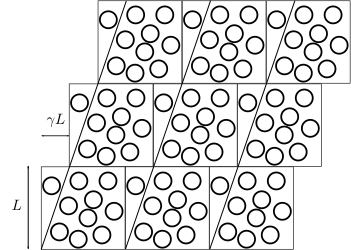
\includegraphics[width=0.6\textwidth]{LeesEdwards.pdf} 
\caption{Schematic two-dimensional representation of the Lees-Edwards boundary conditions. The spatial arrangement of the particles can be interpreted in two ways: as particles \label{fig:LeesEdwardsBoundaryConditions} in square boxes displaced by some offset $\gamma L$ or as aligned boxes tilted by $\theta = \arctan \gamma$.}
\end{figure}

In the Lees-Edwards boundary conditions the image boxes (and the particles included in them) are displaced during the simulation.\\
Simulation of deformation can be performed in several ways. In what follows we outline two possible approaches, differing by the role played by temperature $T$ and shear rate $\dot{\gamma}$.

\subsubsection{Simulation of deformation at $T \neq 0$ and $\dot{\gamma} \neq 0$}
In finite shear rate simulation, particles in the image boxes do drag those at the boundaries with some drift velocity $\dot{\gamma} L$ (where $\dot{\gamma}$ depends on the increment of $d\gamma$ that is applied to the system at each $dt$ molecular dynamics step) so that a velocity profile can be imposed to the system. Particles that cross the boundaries between images with non-zero relative velocity need to be re-inserted in the box at a position that depends on the value of strain $\gamma$ and a velocity that depends on the difference in velocity between the box images \cite{evans2008statistical}. Furthermore, by driving images by imposing a finite strain rate $\dot{\gamma}$ work is done on the system, and is rapidly converted into kinetic energy. A coupling with a thermostat is thus necessary if the system is to be kept at a constant temperature $T$ \cite{evans2008statistical}. Several schemes of this kind have been devised to simulate systems at non-zero $T$ and  $\dot{\gamma}$ and thus recover their transport coefficients, but their application lies outside the scope of this thesis. \\
Furthermore, one of the current limitations of these methods is that low shear rates are not easily accessible. This is because $dt$, if measured in real units and in the case of atomic solids, has to be very small (in the order of femtoseconds) in order to integrate properly the equation of motions of the atoms, and the maximum number of MD steps that can be performed in a reasonable timeframe (roughly in the order of weeks) is around $\approx 10^{9}$ with the computing power available nowadays \cite{voter2002extending}. The consequence is that timescales reachable by MD lie in the microsecond range. Parallelization of ordinary MD algorithms can be successfully used to study \emph{larger} systems, but not to access \emph{longer} timescales. It's then clear that trying to simulate a shear deformation with low strain rate means choosing a $d\gamma$ so tiny that the overall total strain $\gamma$ reachable during the simulation is too small to be useful. Such limitation can be overcome by employing the athermal quasi-static deformation method described below.

\subsubsection[Simulation of deformation at $T = 0$ and $\dot{\gamma} \approx 0$]{Simulation of athermal quasi-static deformation (AQS) at $T = 0$ and $\dot{\gamma} \approx 0$}
The athermal-quasi static (AQS) deformation procedure has been proposed in \cite{tanguy2002continuum} and \cite{maloney2006amorphous}, following earlier methods used in \cite{kobayashi1980computer} to overcome the shear rate limitations of ordinary MD, and it is the method of choice in this work.
Within this approach particle velocities are completely disregarded. An undeformed system ($\gamma = 0$) is initially in an inherent structure, obtained typically by means of an energy minimization procedure. Afterwards, a strain increment of $d\gamma$ is imposed on the system through Lees-Edwards boundary conditions by displacing the upper and lower image boxes in \autoref{fig:LeesEdwardsBoundaryConditions} and by applying the transformation in \autoref{eq:ShearDeformationMatrix}. This has the effect of putting the system in a configuration that does not correspond to an energy minimum anymore. Finally, the system is drawn to a new inherent structure by another application of the energy minimization procedure.  The operations above can then be repeated so to reach arbitrary values of strain in steps of $d\gamma$.
This method turns out to be a reasonable model for systems satisfying two conditions:
\begin{enumerate}
\item Temperatures are low enough so that systems can be imagined as ``rattling'' around a single inherent structure. As this condition satisfied in the limit where $T \rightarrow 0$, this means that the system can be considered athermal.
\item Shear rates are low enough so that, once deformed, the system has time to relax to an inherent structure before further deformation is applied. Being this condition satisfied in the limit where $\dot{\gamma} \rightarrow 0$, one can consider the systems as deformed in a quasi-static way\footnote{the deformation is thus ``adiabatic'', in the same spirit of the adiabatic approximation of quantum mechanics}.
\end{enumerate}
Summarizing, the athermal quasi-static protocol represents the dynamics of glassy system at vanishingly low $T$ and $\dot{\gamma}$.

\section{Simulation of athermal quasi-static deformation \label{sec:LJDeformation}}

\subsection{Effect of deformation on the energy landscape}

The shape of the energy landscape of a system of $N$ particles in a simulation box is dictated by \autoref{eq:TotalPairwiseAdditivePotentialEnergy} and \ref{eq:BinaryLennardJonesPotential} and the boundary conditions. These in turn depend on the shape and volume of the box and on the spatial arrangement of the image boxes (see \autoref{fig:ParticlesInFields}). All these ingredients, in fact, contribute to shaping the exact form of the term $\Delta U$ that must be added to the expression of $U$ in \autoref{eq:TotalPairwiseAdditivePotentialEnergy} (the energy that the particles would have if they were isolated in space) to get the total energy. 

What is the effect of deformation on the energy landscape of a set of particles contained in a simulation box connected to image boxes via Lees-Edwards boundary conditions? Image boxes can be regarded as sources of an external field for the particles located at coordinates $(\mathbf{r_{1}, \ldots, r_{N}})$ in the simulation box, as in \autoref{fig:LeesEdwardsBoundaries}. As the value of the offset in position $\gamma L$ is changed, such external field is modified. This means that the value of the total potential energy is dependent on $\gamma$, and can be thus rewritten as $U(\mathbf{r_{1}, \ldots, r_{N}}, \gamma)$.
The effect of deformation can be thought of, in general, as altering the topology of the energy landscape\footnote{An intuitive picture of this is the effect of erosion/morphogenesis of the surface of the Earth.}. Some of the peaks and minimas of the landscape are thus changed by deformation, while some others are stable. The relevance of the changes of a given feature of the landscape is determined by the importance of the interactions of particles located at the boundaries of the simulation box with respect to those located in the bulk. This can be clarified with an example: consider a configuration such that two particles located deep inside the simulation box have their centers very close together. Due to the repulsive part of the pair potential in \autoref{eq:BinaryLennardJonesPotential} the contribution given by such a pair of particles to the potential energy in \autoref{eq:TotalPairwiseAdditivePotentialEnergy} is very high, so to make this configuration close to a ``peak'' in the landscape. As the particles are not close to the boundaries, there is no way through which a change in the strain (by varying the $\gamma$ in the Lees-Edwards boundary conditions) can change their relative distance, so that such configuration will always be close to a peak in the landscape, regardless the value of $\gamma$. Conversely, a peak due to close particles located in different image boxes can be eroded by deformation, because a change in the strain can separate them and thus reduce the value of their contribution to the total potential energy. Also, a configuration of relatively low energy for some value of the strain can become a peak in the landscape if, by varying $\gamma$, two particles at the boundaries come very close to each other.

\subsubsection{Evolution of inherent structures under deformation}
What's the fate of an inherent structure and its basin under deformation? For a given value of the strain $\gamma$, the energy landscape is fixed and presents a certain number of inherent structures $\mathbf{R_{1}^{*}, \ldots, R_{M}^{*}}$ (where each $\mathbf{R_{i}^{*}}$ stands for a $3N$-dimensional vector of the form $(\mathbf{r_{1}, \ldots, r_{N}})$). For a different value $\gamma'$ the number of inherent structures  $\mathbf{R_{1}^{*'}, \ldots, R_{L}^{*'}}$ won't be the same, because some structures get created or destroyed as the landscape changes as $\gamma$ is varied. In what follows we will identify inherent structures of the landscapes associated to the values of the strain $\gamma$ and $\gamma'$ if, in the $3N+1$-dimensional space (configuration space + strain dimension $\gamma$), there is a path connecting them such that each point in the path is an inherent structure for some value of the strain between $\gamma$ and $\gamma'$ (see \autoref{fig:LifeOfInherentStructures}). We name ``surviving'' or ``stable'' inherent structures those in the sets $\{\mathbf{R_{1}^{*}, \ldots, R_{M}^{*}}\}$ and $\{\mathbf{R_{1}^{*'}, \ldots, R_{L}^{*'}}\}$ that are connected with such a path; we call ``destroyed'' those in the set $\{\mathbf{R_{1}^{*}, \ldots, R_{M}^{*}}\}$ that are not connected with a path to any of those in $\{\mathbf{R_{1}^{*'}, \ldots, R_{L}^{*'}}\}$, and ``created'' those in the set $\{\mathbf{R_{1}^{*'}, \ldots, R_{L}^{*'}}\}$ which are not connected to any of those in $\{\mathbf{R_{1}^{*}, \ldots, R_{M}^{*}}\}$. In \autoref{fig:LifeOfInherentStructures} each inherent structure follows a path in the $3N + 1$ dimensional space.  

\begin{figure}[!h] 
\centering 
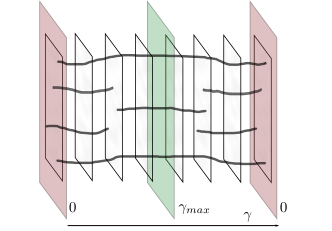
\includegraphics[width=0.6\textwidth]{InherentWorldLines.pdf} 
\caption{Schematic representation of the evolution of energy landscape in a ``configuration space - $\gamma$'' diagram during a shear deformation semicycle. In this picture configuration spaces associated to a given value of $\gamma$ are assumed to be two-dimensional, and each of them has a set of minima (indicated with black dots). As $\gamma$ is increased and the landscape deforms the inherent structures will move in configuration space, tracing the trajectories represented in gray (to avoid clutter, only some of them are shown). Sometimes the inherent structures get destroyed, so that the lines are interrupted; conversely, as new local minima are formed, new trajectories are generated. Due to the reversal of the strain, the diagram is symmetric with respect to the plane of $\gamma = \gamma_{max}$. \label{fig:LifeOfInherentStructures}}
\end{figure}

What does determine the destruction of an inherent structure? Under strain the basin pertaining to a given inherent structure can shrink due to the changes in the landscape, with the inherent structure being closer and closer to the boundaries of the basin. The inherent structure (together with its basin) disappears upon colliding with a saddle point of the landscape \cite{malandro1999relationships}. Such collision has a corresponding hallmark in the Hessian matrix of the potential energy calculated at the inherent structure: right before the collision at least one of the eigenvalues of the Hessian matrix falls to zero \cite{malandro1999relationships}. The creation of an inherent structure is simply the inverse process of the destruction, and these two processes are represented schematically in \autoref{fig:InherentStructureDestructionCreation}.

\begin{figure}[!h] 
\centering 
\includegraphics[width=0.35\textwidth]{inh-016.png} 
\includegraphics[width=0.35\textwidth]{inh-020.png} \\
\includegraphics[width=0.35\textwidth]{inh-023.png} 
\includegraphics[width=0.35\textwidth]{inh-024.png} 
\caption{Schematic two-dimensional representation of the evolution of inherent structures changing the value of $\gamma$. This figure can be seen as a series of projections (or cuts at fixed values of $\gamma$) of the diagram in \autoref{fig:LifeOfInherentStructures}. As $\gamma$ is varied, the energy landscape (represented by equipotential lines) changes and the inherent structures (black dots) move, or get destroyed or created accordingly. \label{fig:InherentStructureDestructionCreation}}
\end{figure}

The destruction of an inherent structure can be also easily visualized in terms of the disconnectivity graphs introduced in \autoref{ch:Introduction}. During deformation, the disconnectivity tree of the landscape gradually changes, with leaves disappearing (as inherent structures and their basins are destroyed) and others forming, and connectivity between them changing.
In particular, the process of destruction of a given inherent structure corresponds to the gradual shortening and final disappearance of the leaf associated to it in the graph.

\subsection{Consequences for athermal dynamics \label{sec:AQSDynamics}}
The way in which the energy landscape evolves during a deformation is intimately related to the evolution of a given starting state under the AQS protocol. For clarity this relationship is schematically illustrated in \autoref{fig:AQSsteps}, and can be analyzed at every elementary operation performed in an AQS step.

\begin{figure}
	\centering
	\begin{subfigure}[b]{\textwidth}
		\centering
		\includegraphics[width = 0.35\textwidth]{aqsstep-020.png}
		\caption{\label{fig:AQSStart}}
	\end{subfigure} \\
	\begin{subfigure}[b]{\textwidth}
		\centering
		\includegraphics[width = 0.35\textwidth]{aqsstepunmin-023.png}
		\caption{\label{fig:AQSUnstable}}
	\end{subfigure} \\
	\begin{subfigure}[b]{\textwidth}
		\centering
		\includegraphics[width = 0.35\textwidth]{aqsstep-023.png}
		\caption{\label{fig:AQSEnd}}
	\end{subfigure} 
	\caption{In this two-dimensional diagram the steps constituting AQS dynamics are represented. The system initially occupies an inherent structure (\subref{fig:AQSStart}). Subsequently, in (\subref{fig:AQSUnstable}), as the strain is increased by $d\gamma$, the landscape is deformed and the system is affinely deformed and is not in an energy minimum anymore. Another step of energy minimization allows to bring the system to a stable minimum (in this case, to the ``same'' inherent structure in the deformed landscape) again in (\subref{fig:AQSEnd}), and another AQS cycle can start again.
	\label{fig:AQSsteps}}
\end{figure}

\begin{enumerate}[(a)]
\item In the AQS protocol a system is initially in an inherent structure configuration (see \autoref{fig:AQSStart}). 
\item An affine map of the kind in \autoref{eq:ShearDeformationMatrix} is applied to the coordinates by setting the incremental strain to $d\gamma$. 
At the same time, boundary conditions between the different images are accordingly updated, so that the energy landscape is slightly changed. In general, the new configuration won't be in a local minimum of the new modified landscape anymore, but slightly away from it\footnote{In this context, it's useful to note that $d\gamma$ plays a crucial role in AQS dynamics. If too large, the deformation of the landscape is dramatic (so that the correlation between the landscapes before and after the deformation is low) and the configuration is fired away in configuration space by the affine transformation, possibly jumping over several valleys and peaks. This is clearly not what AQS is supposed to do, as the system is supposed to follow the changes in the landscape in an ``adiabatic way''. So $d\gamma$ has thus to be small enough to gradually decorrelate the energy landscape and gradually move the system with respect to the lengthscales of the features of the energy landscape in configuration space.} (\autoref{fig:AQSUnstable}).
\item A minimization routine is employed to bring the system back to an inherent structure of the deformed landscape (\autoref{fig:AQSEnd}), and the procedure can be repeated.
\end{enumerate}

During AQS deformation the system thus ``travels'' in configuration space in two different ways, represented schematically in \autoref{fig:AQSEvolution}:

\begin{figure}[!h]
	\centering
	\begin{subfigure}[b]{0.45\textwidth}
		\centering
		\includegraphics[width = 0.8\textwidth]{aqs-016.png}
		\caption{\label{fig:AQSContinuousStart}}
	\end{subfigure} 
	\begin{subfigure}[b]{0.45\textwidth}
		\centering
		\includegraphics[width = 0.8\textwidth]{aqs-020.png}
		\caption{\label{fig:AQSContinuousMiddle}}
	\end{subfigure} \\
	\begin{subfigure}[b]{0.45\textwidth}
		\centering
		\includegraphics[width = 0.8\textwidth]{aqs-023.png}
		\caption{\label{fig:AQSContinuousEnd}}
	\end{subfigure} 
	\begin{subfigure}[b]{0.45\textwidth}
		\centering
		\includegraphics[width = 0.8\textwidth]{aqs-024.png}
		\caption{\label{fig:AQSTransition}}
	\end{subfigure}
	\caption{
	Schematic representation in 2D of the two ways in which a system can move in the energy landscape via AQS dynamics. From (\subref{fig:AQSContinuousStart}) to (\subref{fig:AQSContinuousEnd}) the system moves in a continuous way following a single inherent structure as it evolves. When moving from (\subref{fig:AQSContinuousEnd}) to (\subref{fig:AQSTransition}), however, the inherent structure ceases to exist and the system undergoes a transition to another local minimum.\label{fig:AQSEvolution}}
\end{figure}

\begin{enumerate}
	\item Most of the time (like from (\subref{fig:AQSContinuousStart}) to (\subref{fig:AQSContinuousEnd}) in \autoref{fig:AQSEvolution}), the system sits on the same inherent structure. Increasing the strain makes the inherent structure evolve following a continuous path in the 3$N$+1 dimensional (configuration space + $\gamma$) space, and the system simply follows it through the AQS protocol. As the energy landscape changes gradually, the system moves in the configuration space in a continuous way (that is, to small increments of $\gamma$ correspond small changes in the configuration and in the potential energy). 
	\item At some point (like from (\subref{fig:AQSContinuousEnd}) to (\subref{fig:AQSTransition}) in \autoref{fig:AQSEvolution}), increasing the strain can destroy the inherent structure the system is in, and thus the latter is not in a stable point of the energy landscape anymore. Taking a further AQS step brings the system into the basin of \emph{another inherent structure} and the minimization procedure makes the system reach it. In this case, just one small increment in $\gamma$ is sufficient to make the system reach its \emph{spinodal limit} and jump to a far minimum in configuration space and make it lose abruptly a lot of its potential energy (this is somewhat similar to what happens to a rock brought in small steps on the top of a hill. It can happen that at some point a small step is sufficient to put the rock in an unstable position so that it rolls down the hill\footnote{Don't be mislead by the metaphor though: here it's the \emph{landscape itself} that is altered by the change in strain!}). We will refer to this event as to a \emph{transition}.
\end{enumerate}

The AQS dynamics of a system initially residing in an inherent structure can be represented in terms of ``configuration space - $\gamma$'' diagrams as that reported in \autoref{fig:LifeOfInherentStructures}. With that viewpoint, the inherent structure acts as a ``skeleton'' over which the dynamics of an actual system takes place, as displayed in \autoref{fig:LifeOfASystem}.

\begin{figure}[!h] 
\centering 
\includegraphics[width=0.6\textwidth]{InherentWorldLinesPath.pdf} 
\caption{Representation of the trajectory (in red) of a system in the ``configuration space - $\gamma$'' diagram of \autoref{fig:LifeOfInherentStructures} subjected to a deformation semicycle. The system resides in an inherent structure until such structure is destroyed under the effect of strain. At the values of the strain at which the destruction takes place, the system undergoes an abrupt transitions to other inherent structures.\label{fig:LifeOfASystem}}
\end{figure}

It is possible to look at the athermal dynamics using the viewpoint of disconnectivity graphs also. 
In AQS dynamics, a system resides always on a leaf of a disconnectivity graph. As strain is changed, that leaf can shorten and disappear, as the inherent structure gets destroyed. Just before disappearing, the system resides on a leaf which is very close to an internal vertex of the system, which in turn has different leaves connected to it. At the transition, the leaf where the system is in disappears and the the system falls into one of the leaves\footnote{The number of possible leaves depends on the order of the saddle point associated to the internal vertex.} connected to the internal vertex. 

The way in which the system rearranges right after a transition depends on the region of the landscape where the system is in. 
Rearrangements involving a small number of particles are called in the literature ``shear transformations''. Those involving a large number of particles that scales with the size of the system are called ``avalanches'' instead, and have been interpreted as sequences of shear transformations triggering other shear transformations \cite{bailey2007avalanche, rodney2011modeling}. 

\subsection{Oscillatory athermal deformation}
Via the AQS protocol (or other procedures of simulation of deformation) one can change the strain (in steps) in an arbitrary way. The kind of deformation that is employed in this thesis is \emph{oscillatory}: $\gamma$ is incremented/decremented in steps of $d\gamma$, and has a triangle wave profile varying in the interval $[-\gamma_{max}, \gamma_{max}]$ if plotted against the number of AQS steps (see \autoref{fig:TriangleWave}).

\begin{figure}[!h] 
\centering 
\includegraphics[width=0.8\textwidth]{Triangle.pdf} 
\caption{In the AQS oscillatory strain simulations performed in this thesis, the relationship between the strain $\gamma$ and the \emph{accumulated} strain $\gamma_{acc}$ (i.e. the sum of the absolute incremental strains applied to the system, see \autoref{eq:AccumulatedStrain}) has a triangle wave profile, oscillating in the interval $[-\gamma_{max}, \gamma_{max}]$. \label{fig:TriangleWave}}
\end{figure}

A useful measure of the ``total strain'' applied to a system during an oscillatory deformation experiment is the accumulated strain $\gamma_{acc}$, which can be written as
\begin{equation}
	\gamma_{acc} = \sum_{i} |d\gamma|
	\label{eq:AccumulatedStrain}
\end{equation}

where the $d\gamma_{i}$'s are the incremental strains applied to the system during the deformation, so that $\gamma = \sum_{i} d\gamma$ (without taking the absolute value). Clearly $\gamma_{acc}$ is a monotonic function of the number of steps.
 
From what has been said above, a cyclic deformation alters the initial undeformed landscape until the strain reaches the value $\gamma_{max}$. Then deformation is reversed and the landscape revisits the shapes assumed in correspondence of identical values of $\gamma$, until it finally gets back to its initial form as $\gamma = 0$. The same thing happens as $\gamma$ is varied from 0 up to $-\gamma_{max}$ and then again back to $0$. It's illuminating to focus on the evolution of the inherent structures during such a cyclic modification of the landscape. This is illustrated in \autoref{fig:LifeOfInherentStructuresCycle}. Starting from such a visualization of the evolution of inherent structures like that in \autoref{fig:LifeOfInherentStructuresCycle}, in \autoref{sec:TransitionMatrixModel} we build the TM model of the athermal dynamics of a deformed system.

\begin{figure}[!h] 
\centering 
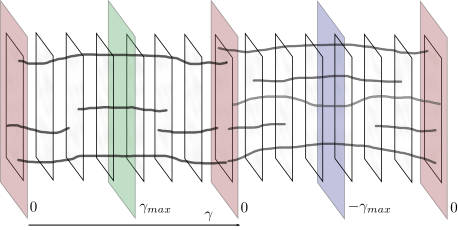
\includegraphics[width=0.9\textwidth]{InherentWorldLinesFull.pdf} 
\caption{Diagram representing the evolution of inherent structures during a full deformation cycle. It is the juxtaposition of two diagrams like that of \autoref{fig:LifeOfInherentStructures}. Note how the two halves of the diagram are symmetric with respect with the planes at $\gamma = \gamma_{max}, -\gamma_{max}$, but the overall diagram is \emph{not} symmetric with respect to the $\gamma = 0$ plane in the middle of the cycle. \label{fig:LifeOfInherentStructuresCycle}}
\end{figure}

